\section{BJT used as a Switch}
For a given BJT circuit, determine $R_1$ and $R_2$ to have $I_C$ saturated at 50mA. In this saturation mode, $V_{CE(Sat)}$ is 30mV. Assume that $V_{BE}$ = 0.7V and the current gain $\beta$ = 100.
-
\begin{figure}[!htp]
    \centering
    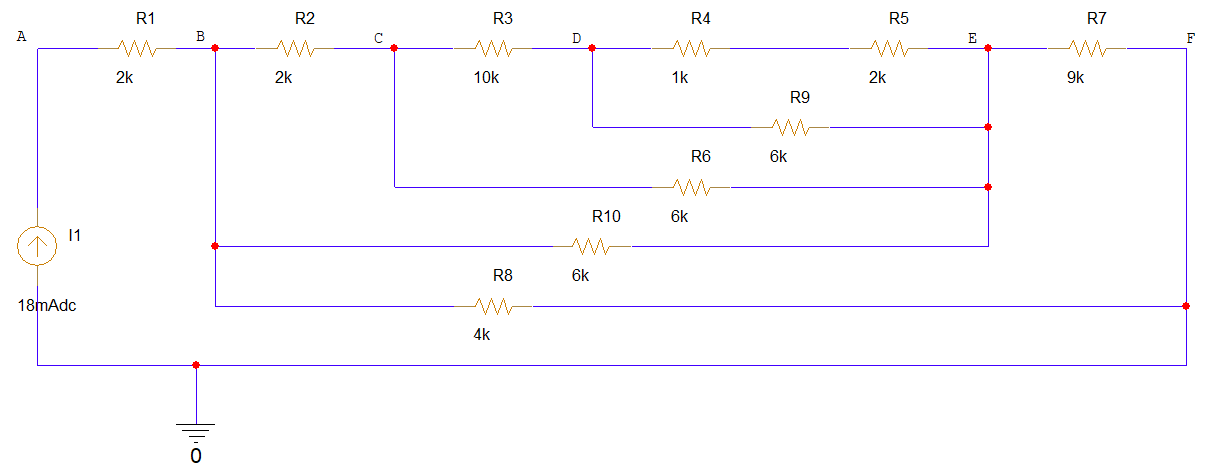
\includegraphics[width=1\linewidth]{graphics/ex3/f1.PNG}
    \caption{\textit{BJT used as switch in saturation mode}}
\end{figure}

Present your solution to determine $R_1$ and $R_2$.
Perform the simulation in PSpice to confirm the results. Capture the screen in PSpice and present in the report.

\textbf{Lời giải:}
\begin{itemize}
    \item $I_B = \frac{I_C}{\beta} = \frac{50mA}{100} = 0.5 mA$

    \item $R_1 = \frac{V_{BB} - V_{BE}}{I_B} = \frac{5V - 0.7V}{0.5 mA} = 8600 \Omega $

    \item $R_2 = \frac{V_{CC} - V_{CE(Sat)}}{I_C} = \frac{10V - 0.03V}{50 mA} = 199.4 \Omega $
\end{itemize}

\newpage
\textbf{\textit{Ảnh mô phỏng:}}\\
\begin{figure}[!htbp]
    \centering
    
    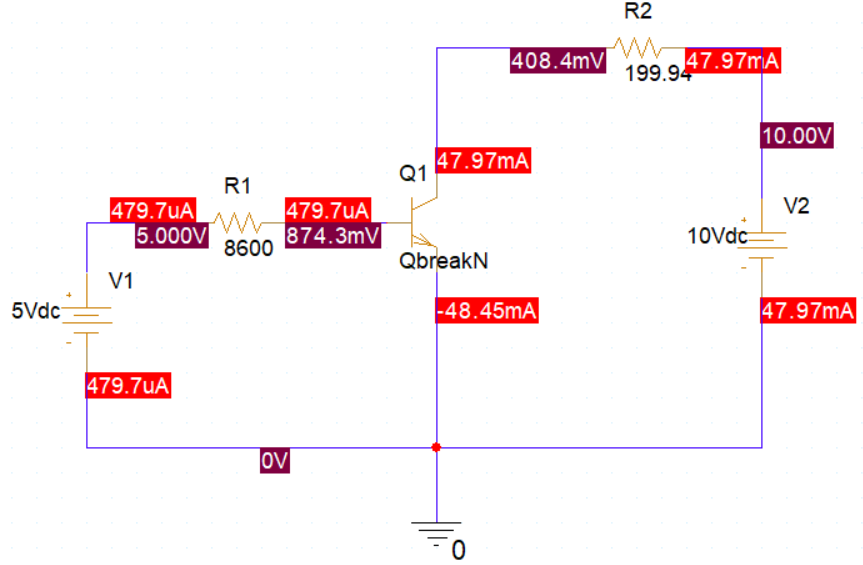
\includegraphics[width=1\linewidth]{graphics/ex3/f2.png}
    % \vspace{6cm}
\end{figure}
